\documentclass[12pt,a4paper,oneside]{report}
\usepackage{enumitem}
\usepackage{xcolor}
%\usepackage{sectsty}
\usepackage{longtable}
\usepackage{caption}
\usepackage{subcaption}
\usepackage{float}
\usepackage{graphicx}
\usepackage{tabularray}
\usepackage{array}
\usepackage{setspace}
\usepackage{tocloft}
\usepackage[nottoc]{tocbibind}
\usepackage{amsmath}
\usepackage{amsfonts}
\usepackage{amssymb}
\usepackage{makeidx}
\usepackage{multirow}
\usepackage[left=1in,right=1in,top=1in,bottom=1in]{geometry}
\usepackage[super,square,sort,comma,numbers]{natbib}
\usepackage[version=4]{mhchem}

%\chapternumberfont{\normalsize} 
%\chaptertitlefont{\LARGE}
%\sectionfont{\large}

\setlength{\extrarowheight}{2pt}

\renewcommand{\thefootnote}{\fnsymbol{footnote}}
\renewcommand{\contentsname}{\Large CONTENTS}
\renewcommand{\cftfigfont}{Figure }
\renewcommand{\cfttabfont}{Table }
\renewcommand{\cftdot}{}
\graphicspath{{./images/}}

\setcitestyle{square}
\pagenumbering{roman}
\date{}

\begin{document}
\thispagestyle{empty}
\begin{center}
{\Large  \MakeUppercase{\bf Automation of DevOps Processes}\\} 
\vspace{0.8cm}
{\Large  \MakeUppercase{\bf Long-Term Internship Report}\\}
\doublespacing
\vspace*{2.5cm}
{\normalsize \it A report submitted in partial fulfillment of the requirements for award of the Degree of\\
}
{\bf BACHELOR OF TECHNOLOGY }\\
{\bf in }\\
{\bf COMPUTER SCIENCE ENGINEERING }\\
{\bf by }\\
\vspace*{1cm}
{\bf\textcolor{blue} {BALINENI SREEDHAR NAIDU }}\\
{\bf \textcolor{blue}{ID: N180058}} \\
{\bf Under supervision of }\\
{\bf Mr. Venkata Narasimha Kowru, SaYukth}\\
{\bf Technologies Pvt Ltd,Hyderabad} \\
{\bf 01 Aug, 2023 to 15 Mar, 2024} \\ 
{\bf Major Project Guide: Mr. Kalapala Sravan Kumar } \\

\vspace*{0.8cm}
\begin{figure}[hbt]
\centering
\vspace*{0.6cm}
\centerline{
\includegraphics[scale=0.29]{images/rgukt.png}}
\end{figure}
\vspace*{0.3cm}
{\small \bf DEPARTMENT OF COMPUTER SCIENCE ENGINEERING}\\
{\small \bf RAJIV GANDHI UNIVERSITY OF KNOWLEDGE TECHNOLOGIES}\\
{\small \bf NUZVID, INDIA\\ }
\end{center}
\newpage
\thispagestyle{empty}
\vspace*{1cm}
\begin{center}{\large \bf DECLARATION}\end{center}
\vspace{1cm}
\setstretch{1.5}
\hspace{1cm}I, \textbf{Balineni Sreedhar Naidu}  hereby declare that the long-term project report is submitted for partial fulfilment of the requirements for the award of the degree of Bachelor of Technology in Computer Science Engineering of the Rajiv Gandhi University of Knowledge Technologies, Nuzvid is a bonafide work done by me under the supervision of\\ \textbf{Mr. Venkata Narasimha Kowru}, Team Leader at SaYukth Technologies Pvt Ltd, Hyderabad, and under the guidance of \textbf{Mr. Kalapala Sravan Kumar }. This submission represents my ideas in my own words and where ideas or words of others have been included, I have adequately and accurately cited and referenced the original sources. I also declare that I have adhered to the ethics of academic honesty and integrity and have not misrepresented or fabricated any data or idea or fact or source in my submission. I understand that any violation of the above will be a cause for disciplinary action by the institute and/or the University and can also evoke penal action from the sources which have thus not been properly cited or from whom proper permission has not been obtained. This report has not been previously formed as the basis for the award of any degree, diploma, or similar title of any other University.
\\
\vspace{1cm} \\
...............................\\
Internal Examiner :\\
Date : \\
\vspace{1cm} \\
\textbf{Balineni Sreedhar Naidu (N180058)}  



\newpage
\pagenumbering{roman}
\thispagestyle{empty}

\setstretch{1.25}
\begin{center}
{\large \bf DEPARTMENT OF COMPUTER SCIENCE ENGINEERING}\\
{\large \bf RAJIV GANDHI UNIVERSITY OF KNOWLEDGE TECHNOLOGIES,}
{\large \bf NUZVID, INDIA}\vspace{0.1cm}\end{center}

\begin{figure}[hbt]
\centering
\centerline{
\includegraphics[scale=0.25]{images/rgukt.png}}
\end{figure}

\begin{center} 
\addcontentsline{toc}{chapter}{Certificate}
{\Large  \textbf{CERTIFICATE}}\end{center}
\begin{spacing}{1.5}
This is to certify that the report entitled \textbf{"Automation of DevOps Processes"} submitted by \textbf{Balineni Sreedhar Naidu (N180058)} to the Rajiv Gandhi University of Knowledge Technologies, Nuzvid in partial fulfilment of the requirements for the award of the Degree of Bachelor of Technology in Computer Science Engineering is a bonafide record of the project work carried out by him under our guidance and supervision. This report in any form has not been submitted to any other University or Institute for any purpose.\end{spacing}
\vspace{2cm}
\noindent
\begin{tabular}[t]{@{}l}
\textbf{Mr. Kumar Anurupam }\\ Internal Supervisor\\Professor\\Dept. of Computer Science Engineering \\RGUKT NUZVID
\end{tabular}
\hfill
\begin{tabular}[t]{@{}r}
\textbf{Mr. R. Siva Narayana}\\External Supervisor\\Asst.Professor\\Dept. of Computer Science Engineering\\RGUKT NUZVID
\end{tabular}



\vspace{2cm}
\noindent
\begin{tabular}[t]{@{}l}
\textbf{Mr. B. Mahalakshmi Rao}\\External Supervisor\\Asst.Professor\\Dept. of Computer Science Engineering\\RGUKT NUZVID
\end{tabular}
\hfill
\begin{tabular}[t]{@{}r}
\textbf{Dr. D.V. Nagarjuna Devi}\\Head of the Department\\Dept. of Computer Science Engineering \\RGUKT NUZVID
\end{tabular}

% \vspace{2cm}
% \noindent
% \begin{tabular}[t]{@{}l} 
% \textbf{Mr. S. Chiranjeevi}\\Head of the Department\\Dept. of Computer Science Engineering \\RGUKT NUZVID
% \end{tabular}
% \hfill
% \begin{tabular}[t]{@{}r} 
% \end{tabular}




\newpage

\thispagestyle{empty}
\vspace*{3cm}
\addcontentsline{toc}{chapter}{Acknowledgement}
\begin{center}  {\large \bf ACKNOWLEDGEMENT}\end{center}
\vspace{1cm}
\setstretch{1.5}
\hspace{1cm}We express our sincere gratitude towards our Team Leader \textbf{Mr.Venkata Narasimha Kowru}, SaYukth Technologies Pvt Ltd, and our guide \textbf{Mr.Kalapala Sravan Kumar},
Computer Science Engineering, Rajiv Gandhi University of Knowledge Technologies for his valuable guidance, suggestions, and supervision throughout the work. Without his patronage and guidance, the project would not have taken shape. We would also like to express our regards for his kind approval of the project, time-to-time counseling, and advice. We owe our sincere thanks to the Dept.of Computer Science Engineering, Rajiv Gandhi University of Knowledge Technologies. 
\newpage
\vspace*{2cm}
\addcontentsline{toc}{chapter}{Abstract}
\begin{center}  {\Large \bf ABSTRACT}\end{center}
\vspace{1cm}
\noindent 
\hspace{1cm}
This project focuses on developing a comprehensive suite of automation scripts tailored for DevOps activities. These scripts are meticulously designed to streamline various facets of DevOps operations, including installation of servers, code deployment via continuous integration and continuous deployment (CI/CD) pipelines, server monitoring and logging, automated security assessments for both source code and system firewalls and back up the data and checking the backups health. By leveraging these automation scripts, organizations can enhance efficiency, reduce manual intervention, and maintain robustness across their DevOps workflows.
\setstretch{1.3}


\newpage
\thispagestyle{empty}

\newpage
\tableofcontents 	
\cleardoublepage 

% \listoftables 	\cleardoublepage 
\listoffigures 	\cleardoublepage

\newpage
\begin{center}  {\Large \bf ABBREVIATIONS}\end{center}
\vspace{1cm}\doublespacing
\begin{tabular}{l l}

CI & Continuous Integration \\
CD & Continuous Deployment  \\
HAProxy & High Availability Proxy \\
SCP & Secure Copy \\
SSH & Secure Shell \\
DNS & Domain Name System \\
URL & Uniform Resource Locator\\



\end{tabular} 

\newpage
\pagenumbering{arabic}
\chapter{Introduction}
DevOps is a software development approach and a cultural shift that focuses on collaboration, communication, integration between, and automation in software development (Dev) and IT operations (Ops). Some core principles of DevOps include collaboration, implementing automation, and adopting continuous delivery practices.  \\
Introducing our proposed method for automating DevOps processes,  facilitates the seamless installation and configuration of our technology stack on servers, enabling rapid deployment, monitoring, and scalability for new projects. By automating these processes, we aim to reduce setup time to mere minutes, ensure easy configuration of clusters without manual intervention, and provide a framework that simplifies upgrades and testing across different stack configurations.\\
\newline
\hspace{1cm} One key aspect of our automation strategy is the separation of configuration variables, which not only enhances stack upgradability but also promotes ease of testing by allowing us to experiment with different stack configurations effortlessly. These automation pipeline encompasses a range of functionalities aimed at streamlining server management and ensuring robustness in operations. This includes the installation of monitoring stacks with pre-configured dashboards and alert rules, enabling proactive alerts via email for any anomalies or unwanted events occurring on the servers. Additionally, these DevOps processes encompass security measures, compliance checks, and Linux hardening practices to fortify our infrastructure against potential threats.\\
\newline
\hspace{1cm} To optimize resource usage and prevent server downtime, our scripts incorporate start and stop scripts that manage service initialization in a sequenced manner, mitigating resource contention issues that could lead to performance bottlenecks.\\
\newline
\hspace{1cm} Furthermore, this automation framework extends to data backup and restoration tasks, ensuring data integrity and providing a mechanism to test the health of backups on alternative servers. Custom monitoring dashboards and exporters are also integrated into our scripts, facilitating comprehensive monitoring of backup data health and overall system performance. This report provides a detailed overview of our automation procedures, including the implementation approach, working mechanisms of various scripts, and the benefits accrued in terms of efficiency, reliability, and scalability in our DevOps workflows.\\



 
\newpage
\chapter{Background and Related Work}

In the realm of DevOps automation, tools such as Puppet, Chef, and Ansible have been extensively utilized to automate server and application configurations. These tools offer both declarative and imperative approaches to define and manage configurations. Puppet, known for its declarative approach, allows users to specify the desired state of a system, while Chef follows an imperative approach where users define the steps to achieve a desired configuration. Ansible, with its agentless architecture and YAML-based playbooks, offers a streamlined way to automate configuration tasks across systems. \\

  While these Configuration Management Tools are widely adopted and effective for managing configurations across diverse systems and applications in data center environments, they may not entirely suit our specific needs.
However, for our project's objectives, which primarily revolve around seamless installation and configuration of technology stacks on servers, these traditional Configuration Management Tools may not provide the level of simplicity, flexibility, and scalability that we require. Our focus is on rapid deployment, easy configuration of clusters, and swift upgrades without manual intervention and setting up monitoring applications stacks along with ensuring security through Linux hardening. This necessitates a tailored approach that provides simplicity, flexibility, and scalability specific to our DevOps workflows and technology stack requirements. \\

By recognizing the strengths and limitations of traditional Configuration Management Tools in previous work, we aim to leverage custom Python scripts and a modular architecture to achieve the desired level of automation and configurability. This approach is designed to align closely with our project's objectives, ensuring efficient deployment, easy cluster configuration, and seamless upgrades, all while minimizing manual intervention and complexity.This project aims to leverage custom Python scripts and a modular architecture to achieve the desired level of automation and configurability, tailored specifically for our DevOps workflows and technology stack requirements.




\newpage
\chapter{Methodology}
To streamline the installation and configuration processes of the required technology stack components, we have developed Python automation scripts that are integrated into a Jenkins pipeline. This integration allows for seamless checkout of the scripts on the server, simplifying the installation process by accepting the application name as a command-line argument for the respective Python script. The scripts are structured in a way that separates resource URLs, version numbers, data directories, firewall ports, and other parameters into distinct files, facilitating easy modification and upgrades of the stack.\\ 

Manually checking out and running these scripts on servers can be a cumbersome task, which is why Jenkins pipelines are utilized to automate these steps. The primary objective of the Jenkins pipeline is to enable one-click installation and configuration of the necessary technology stack components. This streamlined process extends to other applications crucial for developer operations, deployment, and monitoring, all accessible within a few clicks through the Jenkins web console. \\

Additionally, beyond installation and configuration, ensuring the security of servers through Linux hardening and implementing data backups is imperative. Another Jenkins pipeline is dedicated to modifying necessary configurations in the Linux hardening script and executing it on the server. This pipeline also includes steps to expose metrics using an exporter and integrate them into the monitoring stack. By building custom exporters, metrics related to backup and restore state are exposed and visualized in Grafana within minutes, providing real-time insights into the system's health and backup status. This comprehensive automation approach significantly reduces manual efforts, enhances system security, and improves visibility into critical metrics for efficient monitoring and management.









\begin{figure}[ht]
    \centering
    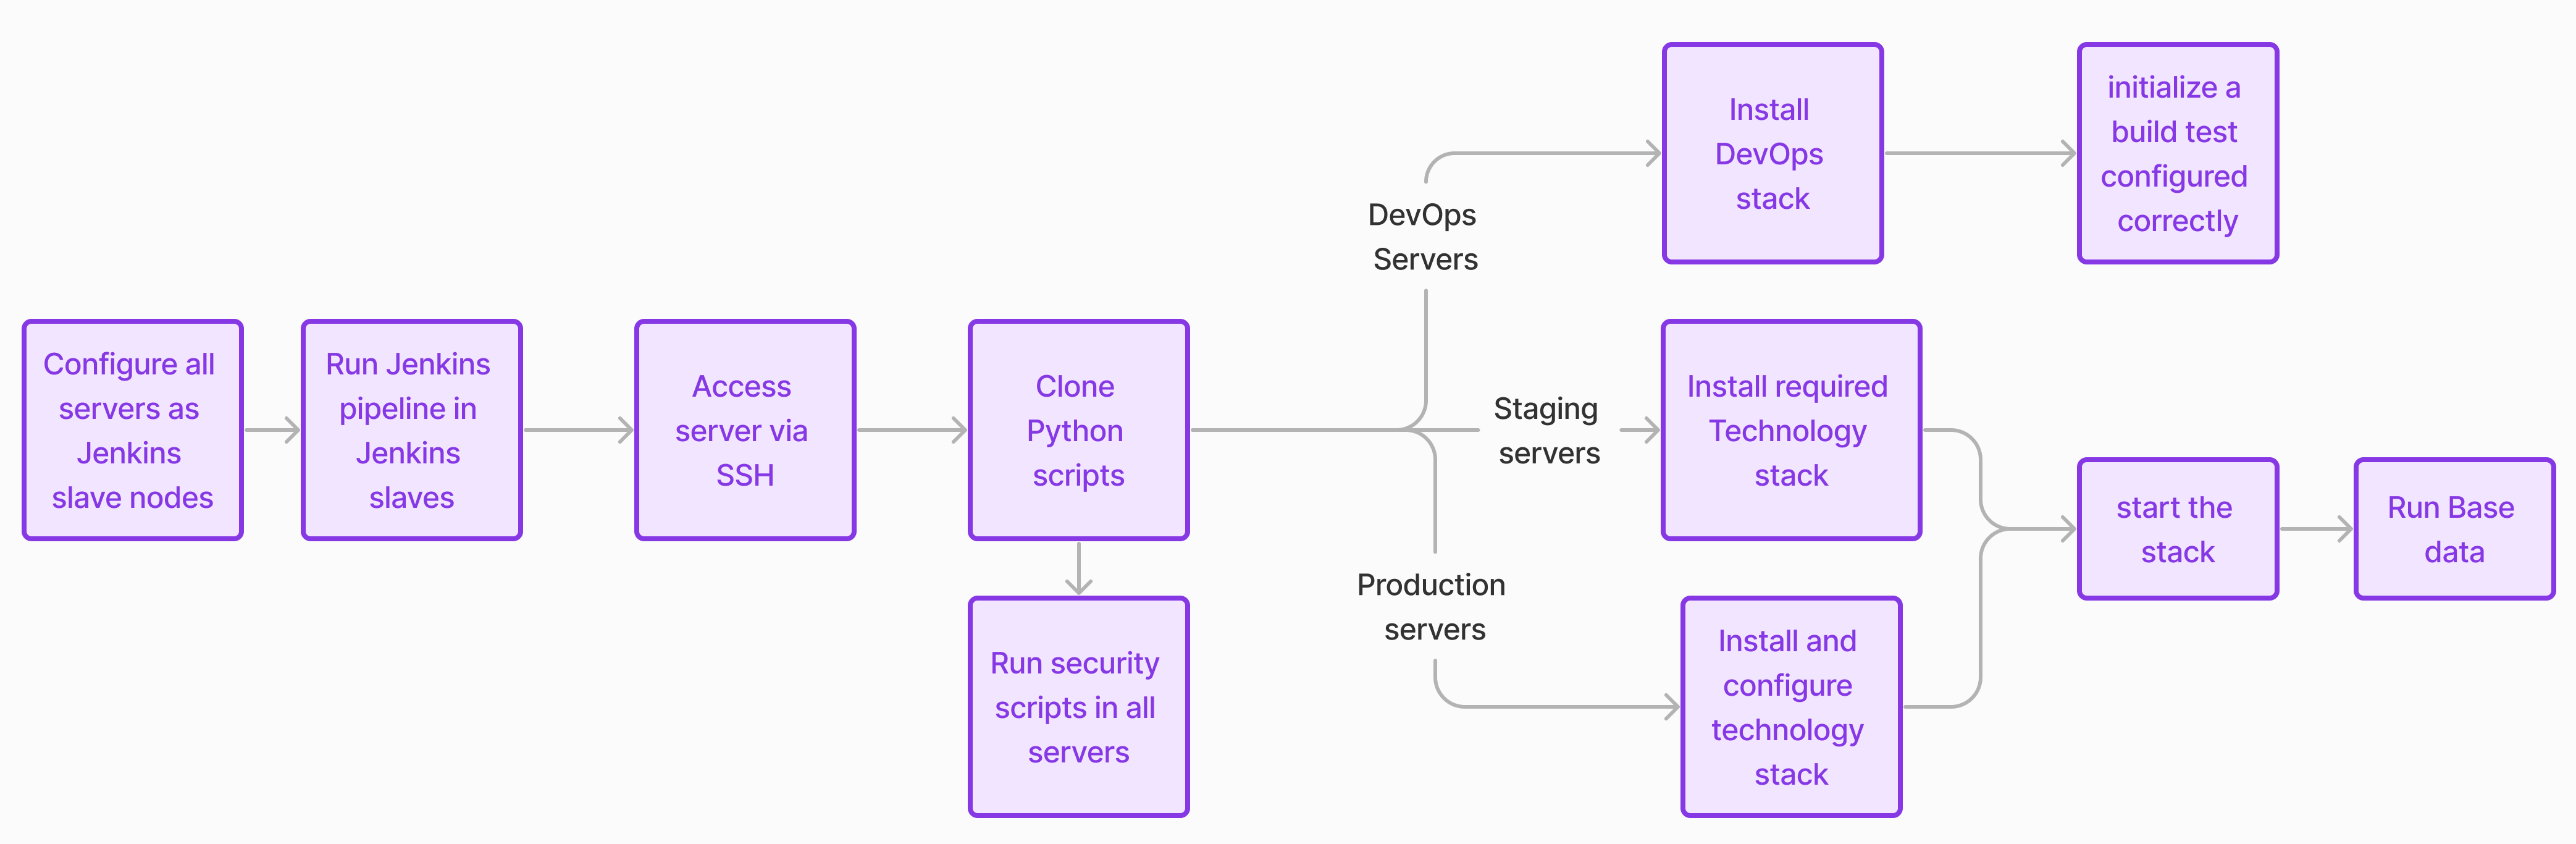
\includegraphics[width= 180mm, height = 80mm]{images/flowchart.png}
    \caption{Flowchart of Automation Processes}
    \label{fig:figure2_2}
\end{figure}
\section{Jenkins}
\par  Jenkins is an open source automation server. It helps automate the parts of software development related to building, testing, and deploying, facilitating continuous integration, and continuous delivery. It is a server-based system that runs in servlet containers such as Apache Tomcat. Jenkins plays a crucial role in automating various processes related to installation, configuration, security, monitoring, and management in DevOps workflows.

\subsection{Integration with Version Control}
\hspace{1cm} Jenkins seamlessly integrates with version control systems like Git, allowing for versioned scripts and configurations. This integration ensures that the latest versions of scripts are pulled from the repository during pipeline execution, promoting version control and traceability.

\subsection{Pipeline Orchestration}
\hspace{1cm} Jenkins pipelines orchestrate the entire process from start to finish. This includes steps such as checking out scripts, installing the necessary stack components, configuring the stack, executing Linux hardening scripts, and setting up data backups. Pipelines ensure that these tasks are executed in a specified sequence, reducing errors and ensuring consistency.

\subsection{Automated Script Execution}
\hspace{1cm} Jenkins facilitates the automated execution of Python automation scripts for installing and configuring the technology stack. By integrating these scripts into Jenkins pipelines, tasks that would otherwise require manual intervention, such as checking out scripts on servers and running them, are automated.


\subsection{One-Click Deployment}
\hspace{1cm} Jenkins enables one-click deployment through its web interface or API. This simplifies the deployment process, allowing users to trigger the entire automation workflow with a single click, as mentioned in the methodology.

\subsection{Monitoring and Visualization}
\hspace{1cm} Jenkins integrates with monitoring and visualization tools like Grafana, allowing for real-time monitoring of system metrics, backup status, and overall system health. This integration enhances visibility into critical metrics and provides insights for effective monitoring and management.

Overall, Jenkins streamlines and automates the DevOps processes involved in installing, configuring, securing, and monitoring technology stacks, making the entire workflow more efficient, reliable, and scalable.



\section{DevOps application stack}
\par The DevOps application stack refers to the integrated set of software tools, technologies, and services used to automate and streamline the development, deployment, monitoring, and management processes within a DevOps environment. The appplications mentioned below need to be installed in DevOps servers.

\begin{figure}[ht]
    \centering
    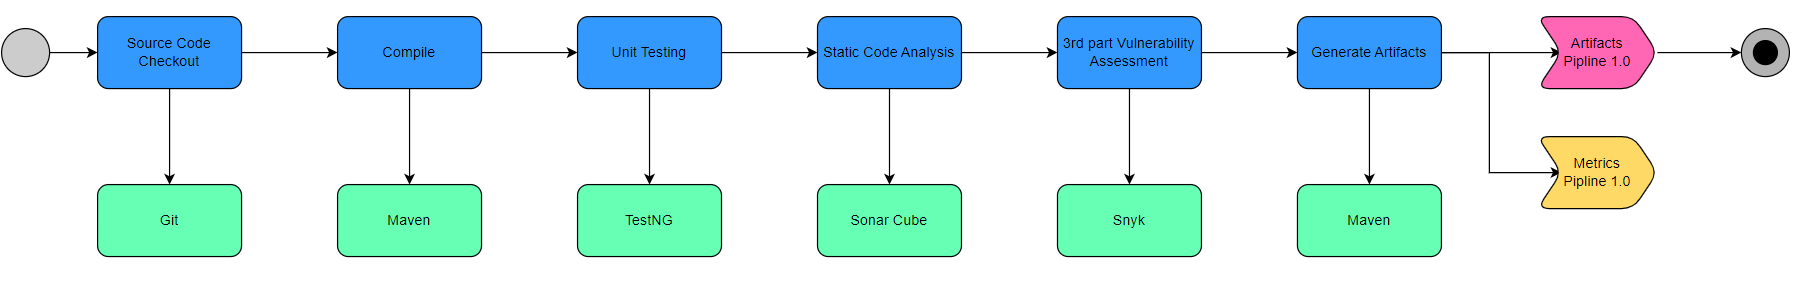
\includegraphics[width=180mm , height = 50mm]{images/devops stack.png}
    \caption{DevOps pipeline}
    \label{fig:figure2_2}
\end{figure}

\begin{itemize}
  


\item \textbf{Git} is a distributed version control system used for tracking changes in source code during software development. It allows multiple developers to collaborate efficiently by managing different versions of files and facilitating merging changes.

\item \textbf{Maven} is a build automation tool primarily used for Java projects to manage project dependencies, build processes, and project lifecycle management. It simplifies the build process by providing a standardized structure, known as Project Object Model (POM), which defines project configuration, dependencies, and build targets. Maven retrieves dependencies from central repositories, allowing developers to easily manage and share libraries across projects. It also supports various plugins for additional functionalities such as testing, packaging, and deployment, making it a popular choice for Java developers for efficient project management and automation.

\item \textbf{TestNG} is a testing framework designed for Java that facilitates the creation and execution of automated tests. It supports a wide range of testing scenarios, including unit, functional, integration, and end-to-end testing. TestNG offers features such as annotations, parameterized testing, test dependency management, and parallel test execution, enhancing test flexibility, readability, and scalability. It is widely used in the Java community for its robust testing capabilities and integration with build tools like Maven and continuous integration platforms like Jenkins.

\item \textbf{SonarQube} is an open-source static code analysis tool used for continuous inspection of code quality and security vulnerabilities. It analyzes code across multiple programming languages, identifying issues such as bugs, code smells, security vulnerabilities, and duplication. SonarQube provides detailed reports, metrics, and visualizations to help developers and teams improve code quality, maintainability, and reliability. It integrates seamlessly into the CI/CD pipeline, allowing for automated code analysis and enforcing code quality standards throughout the development lifecycle.

\item \textbf{PostgreSQL} is used with SonarQube for its scalability, reliability, performance, and security features, ensuring efficient storage and management of code analysis data. SonarQube officially supports PostgreSQL, making it an ideal choice as the database backend for organizations using SonarQube for code quality and security analysis.

 
\item \textbf{Snyk} is a developer-first security platform that helps organizations find, fix, and prevent vulnerabilities in open-source libraries and container images. It scans projects and dependencies for known security vulnerabilities and provides actionable insights to remediate issues. Snyk integrates with CI/CD pipelines to automate vulnerability scanning and remediation, ensuring that vulnerabilities are addressed early in the development process. Its continuous monitoring capabilities help organizations stay updated on new vulnerabilities and maintain a secure codebase.
\end{itemize}

\section{Deployment stack}
\par In this deployment architecture, incoming traffic first passes through a firewall that acts as a security barrier, filtering and allowing only authorized requests to proceed. Behind the firewall, HAProxy, a high-performance load balancer, distributes the incoming traffic across a cluster of Tomcat servers. These Tomcat servers host the application logic and handle client requests efficiently. The communication between HAProxy and the Tomcat server cluster is optimized for load balancing and fault tolerance, ensuring that the workload is evenly distributed and that the system remains highly available. Additionally, the Tomcat servers are interconnected with Percona XtraDB Cluster, ScyllaDB Cluster, and Redpanda Cluster, forming a robust backend infrastructure for data storage, processing, and messaging. This setup ensures scalability, reliability, and performance for handling diverse workloads and maintaining smooth operations of the overall system.


\begin{figure}[ht]
    \centering
    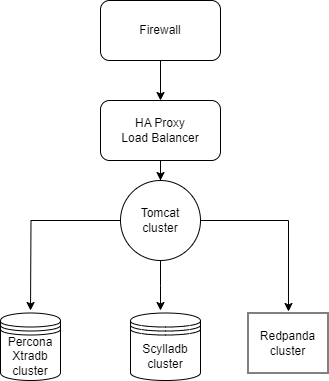
\includegraphics[width=120mm , height = 130mm]{images/deploy.drawio.png}
    \caption{Server Architecture}
    \label{fig:figure2_2}
\end{figure}

\par The main objective is to automate the deployment of this application architecture, including the installation and configuration of databases across multiple servers to form clusters. This automation streamlines the setup process, allowing for easy scaling by adding additional database servers to handle increasing loads efficiently. The focus is on creating a seamless infrastructure where Tomcat servers can dynamically distribute the workload among different database clusters, optimizing performance and ensuring high availability.

\begin{itemize}
\item \textbf{HAProxy} is a high-performance open-source load balancer that efficiently distributes incoming network traffic across multiple backend servers based on customizable rules and algorithms. It helps improve application performance, scalability, and reliability by evenly distributing workloads and managing server resources effectively.

\item \textbf{Apache Tomcat} is an open-source Java-based servlet container that provides a runtime environment for Java web applications. It serves as a web server capable of executing Java servlets and JavaServer Pages (JSP), handling HTTP requests, and generating dynamic content. Tomcat's architecture includes a core servlet container responsible for managing the lifecycle of servlets, along with additional components like Catalina for managing web applications, Coyote for handling HTTP requests, and Jasper for JSP processing, making it a versatile platform for hosting Java web applications.

\item \textbf{Percona XtraDB Cluster} is an open-source, high-availability MySQL clustering solution based on the Percona Server for MySQL. It is designed to provide high performance, scalability, and fault tolerance for database environments. Percona XtraDB Cluster uses synchronous replication between nodes, ensuring data consistency across the cluster while offering automatic node recovery and failover capabilities. Additionally, it supports features like multi-master replication, read and write scalability, and easy integration with existing MySQL applications, making it a robust choice for deploying highly available MySQL databases.

\item \textbf{ScyllaDB} is a distributed NoSQL database built for high performance and low-latency applications. It is designed as a drop-in replacement for Apache Cassandra, providing compatibility with Cassandra Query Language (CQL) and data models while offering superior performance. In a ScyllaDB cluster, data is distributed across multiple nodes for scalability and fault tolerance, with each node capable of handling reads and writes independently. The cluster employs a shared-nothing architecture, where each node operates autonomously and communicates through a gossip protocol for coordination and data replication. ScyllaDB's efficient design and integration with modern hardware technologies make it well-suited for real-time big data workloads and high-throughput applications.
\item \textbf{Redpanda} is a distributed streaming platform designed for high-performance, low-latency, and scalable data processing. It is built as an alternative to Apache Kafka, offering compatibility with Kafka APIs and tools while providing improved performance and reliability. In a Redpanda cluster, data streams are distributed across nodes for fault tolerance and horizontal scalability, making it suitable for real-time data streaming and event-driven applications.
\end{itemize}


\section{Monitoring Stack}
\par The automation process encompasses the installation and configuration of various service exporters such as MySQL, Scylla, Redpanda, PostgreSQL, Node, HAProxy, Jenkins, and others. These exporters facilitate the extraction of specific metrics and data from the respective services, making them accessible to Prometheus for centralized monitoring. Prometheus is then configured to collect metrics from these exporters, apply custom requirement alert rules, and store the data in a dedicated time series database configured to maintain data for at least 365 days. Furthermore, Grafana is automated for installation, and customized dashboards are set up to visualize the collected metrics from Prometheus, enabling effective monitoring and analysis of system performance and health. This end-to-end automation enhances operational efficiency, provides real-time insights, and supports proactive management of the entire infrastructure and services.

\begin{figure}[ht]
    \centering
    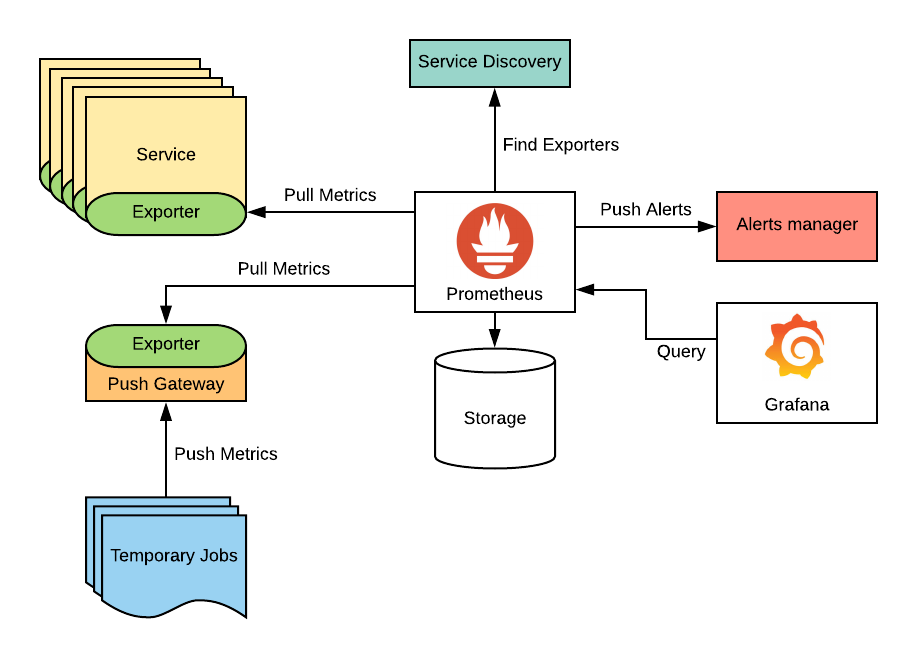
\includegraphics[width=140mm , height = 120mm]{images/monstack.png}
    \caption{Monitoring Stack Architecture}
    \label{fig:figure2_2}
\end{figure}

\begin{itemize}
\item \textbf{Service Exporters: }Service exporters in Prometheus are specialized exporters used for monitoring specific services or applications that don't expose Prometheus-compatible metrics natively. These exporters bridge the gap by translating service-specific metrics into a format that Prometheus can scrape and process. Examples include Node Exporter for system-level metrics, Blackbox Exporter for probing endpoints, and exporters for databases (e.g., MySQL, PostgreSQL) and cloud platforms (e.g., AWS, Azure) to monitor their performance and health metrics within Prometheus.
\item \textbf{Prometheus: }Prometheus is an open-source monitoring and alerting toolkit designed for collecting and processing metrics from various sources. It offers a multi-dimensional data model, powerful querying language (PromQL), and efficient storage for time-series data. Prometheus scrapes metrics from instrumented applications, services, and systems, providing insights into their performance and health.
\item \textbf{Prometheus Alertmanager: }Prometheus Alertmanager is a component that manages and handles alerts generated by Prometheus. It provides features like deduplication, grouping, and routing of alerts to different receivers (e.g., email, PagerDuty, Slack) based on predefined rules and configurations. Alertmanager enhances the monitoring experience by ensuring timely and effective response to critical events and incidents.
\item \textbf{Grafana: }Grafana is an open-source analytics and visualization platform that integrates with Prometheus and other data sources to create interactive and customizable dashboards. It enables users to create visual representations of metrics collected by Prometheus, helping teams to monitor and analyze system performance, identify trends, and gain actionable insights through graphs, charts, and alerts.
\end{itemize}


\section{Linux hardening}
\par Linux hardening involves implementing various security measures to protect a server from potential threats and vulnerabilities. This includes securing network services, managing user permissions, enabling firewall rules, applying system updates regularly, and configuring audit logs. By hardening Linux systems, organizations can reduce the attack surface, mitigate risks, prevent unauthorized access, and enhance overall system security. In the automated process, the Linux system hardening measures are validated using tools like Lynis. Lynis assesses the security posture of Linux systems by evaluating configuration settings, checking for security best practices adherence, and assigning a security score based on the findings. The requirement is that the Lynis score should be more than 85 percent to proceed with setting up the technology stack.

Additionally, the Lynis score is integrated as a metric in Prometheus, which collects and stores system metrics, including the Lynis score. This metric is then visualized in Grafana, providing a comprehensive view of the server's security status. This automated process not only ensures that the server meets security standards but also provides visibility into the security posture through Grafana dashboards, enabling proactive monitoring and management of system security.

 \section{Automating the Data Backup and Restoration}
\par To automate the data backup process in MySQL and ScyllaDB databases, we will schedule nightly backups at 2:00 am using cron jobs or scheduled tasks. These backup scripts will be designed to capture all necessary data and configurations from both MySQL and ScyllaDB databases, ensuring comprehensive backup coverage. Following the backup process, verification checks will be implemented to ensure data integrity. This includes automatically verifying the number of rows in MySQL tables and the number of columns in ScyllaDB tables within the backup files. Automated scripts or queries will handle these verification checks, comparing the counts in the backup files against the corresponding tables in the production databases.

Next, an automated restoration process will be set up on a separate server to restore the production backups of MySQL and ScyllaDB databases. This segregated server environment ensures a non-disruptive restoration process. Once the restoration is complete, another automated comparison will be conducted to verify the row/column counts between the restored databases and the production databases. If the counts match, indicating successful restoration, the metric will be exposed.

However, if discrepancies are detected during the comparison, indicating a potential issue with the restoration process, an alert will be triggered. The alerting mechanism will be integrated with Prometheus for monitoring purposes. In case of a mismatch in row/column counts, an alert will be sent out to all DevOps engineers via email or Slack channels, ensuring prompt notification and resolution of any backup or restoration issues. This comprehensive automation workflow streamlines the data backup, restoration, verification, and monitoring processes, enhancing data reliability and operational efficiency.


\newpage
\chapter{Implementation}
\section{Automating deployment}
\begin{figure}[H]
	\centering
	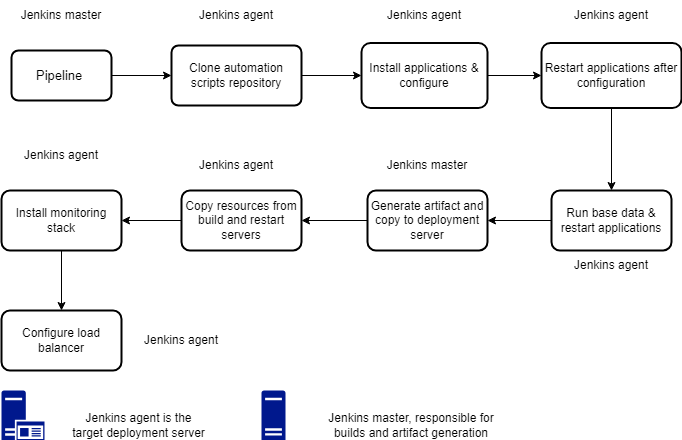
\includegraphics[width=155mm , height = 100mm]{images/jenkins-full.png}
	\caption{Deployment automation architecture}
	\label{fig:figure4_1}
\end{figure}
\textbf{{\large Jenkins}}
\par\hspace{1cm} \textbf{Jenkins} is an open-source automation server widely used for continuous integration (CI) and continuous delivery (CD) pipelines. It provides a platform for automating software development processes, including building, testing, and deploying applications. Jenkins is a key tool in the DevOps ecosystem due to its flexibility, extensibility, and large community support. 
\par\hspace{1cm} Using its "Pipeline as Code" feature, we developed autmation scripts involving intermediate installation and configuration scripts using python. Jenkins Pipeline is written in Groovy, a scripting language that provides a high level of flexibility and expressiveness for defining complex workflows.

\par\hspace{1cm} \textbf{Jenkins Master}, is a terminology used to refer the DevOps server which is used to perform DevOps operations on like builds, artiffact generation. Whenever a build is triggered, if configured to get pipeline from git repository, it clones the repository on master server before progressing through build steps.

\par\hspace{1cm}\textbf{Jenkins Agent/Slave}, is a terminology to refer a deployment server where the application needed to be deployed on. It is usually pre-configured from Jenkins Interface along with credentials to access the remote server. An slave can also be used without pre-configuring it's IP and credentials to be used as a deployment server(For which, pipeline should include all necessary information).


\hspace{1cm}\textbf{{\large Pipeline as code}}
\par\hspace{1cm}Jenkins Pipeline as Code is a concept that changed how software development workflows are managed and executed within Jenkins, an automation server commonly used for continuous integration and continuous delivery (CI/CD) processes. Traditionally, developers would configure their build, test, and deployment tasks manually within the Jenkins user interface. However, with Pipeline as Code, these processes are defined and managed through code, allowing for greater flexibility, repeatability, and scalability in software delivery pipelines.

\par\hspace{1cm} Our approach uses both declarative and scripted pipeline to install, configure, deploy our target application. Pipeline code starts with a "pipeline" block which defines environment variables used for the entire pipeline and agent declaration which concludes if each stage in the pipeline needs to define its custom agent for the script in each step to be run on. The logic for this automation is divided into several stages, each stage performing similar steps aiming to complete the deployment.

\par\hspace{1cm}At its core, Jenkins Pipeline as Code enables developers to define their entire CI/CD workflow in a declarative or scripted format using the Groovy programming language. This workflow script, often referred to as a Jenkinsfile, outlines the stages, tasks, and conditions for building, testing, and deploying applications. By encapsulating the entire pipeline logic in code, teams can version-control, review, and collaborate on their pipeline configurations just like they do with application code.

\subsection{Installation of required application servers}
\par\hspace{1cm} 
In the initial phase of website/application deployment, we automate the optimization of the configuration of the rented server from the cloud provider to meet our requirements. This process involves setting up the node's hostname, configuring timezone. And updating the package manager's repository, installing required language support tools such as python3 and other tools which allows downloading files such as gdown. Additionally, automation is employed to configure the hosts file for the server with it's private IP and cluster names, which acts as a local DNS for a machine, serving as a prerequisite for deployment.
 \par\hspace{1cm} After configuring the server with required specifications, We need to install application servers required by the deploying application such as Percona XtraDB as Relational Database Server,Redpanda as messaging queue, Scylla server as Non-relational database server, Tomcat as a webserver, HAProxy as a loadbalancer. 
\par\textbf{For each application, several parameters are defined to customize, such as:}
\begin{itemize}
	\item Version
	\item Port (for application servers)
	\item Installation path
	\item Download URL/ drive ID(for custom binaries)
	\item Memory limits (for database, webserver)
\end{itemize}
\par\hspace{1cm} All the above parameters are defined in project specific configuration directory with directory identifier starting with project name followed by "ConfigurationFiles". In which, install.conf, configuration.conf files are defined, and for the installation, the script uses parameters which are defined as "paramater = value" format from the install.conf file. And the script splits each line which are not either section headers nor blank lines, into key and values and then declares as variables for usage in the code defining script file. So, the variables are defined on the fly.
\par\hspace{1cm} The isolation of code from parameters help in organizing code and helps for the script executor to easily understand what's happening.

\subsection{Configuring installed application servers}
\par\hspace{1cm}After installing requirede application stack, We need to configure them to work with the application. This step include configuring hosts file with clusternames of mysql, scylla, redpanda with the node's private IP. This step also includes creating required directories for applications for data, for error pages to be returned for load balancer, etc. It also includes changing application's default configuration files to the one's we configured in the configuration.conf file(same format as of install.conf), this process includes changing cluster names, data directories to be used, private IP addresse changes, and some important properties changes such as running mysql in bootstrap mode or running scylla with only limited CPUs. This step also includes changing permissions, ownerships for directories that these applications use. And these permissions needs to be given such that if the service is being started by user root, only root user will have access to the required directories. After configuring, the servers are started to reflect the changes.

\subsection{Artifact generation}
\par\hspace{1cm} An artifact can be seen as a bundled version of code which can be served through application servers specifically designed for the source code language. Such as .war artifact for java based application and .apk for android based applications, .exe for windows applications, etc.

\hspace{1cm}\textbf{{\large Artifact Generation Process}}
\begin{itemize}
	\item \textbf{Fetch source code}: Source code from version control system needs to be first cloned into the devops server after which artifact generation process starts, we use github as our version control system to get source code.
	\item \textbf{Build}: For compiling and building java based web-applications involving spring boot from source code, we use maven tool. And for android based applications, we use gradle as our build tool to generate the artifact.
	\item \textbf{Testing}:
	\begin{itemize}
		 \item \textbf{snyk},is a developer-first security platform that helps organizations find, fix, and prevent vulnerabilities in open-source libraries and container images. It scans projects and dependencies for known security vulnerabilities and provides actionable insights to remediate issues. Snyk integrates with CI/CD pipelines to automate vulnerability scanning and remediation, ensuring that vulnerabilities are addressed early in the development process. Its continuous monitoring capabilities help organizations stay updated on new vulnerabilities and maintain a secure codebase.
	\item \textbf{SonarQube} is an open-source static code analysis tool used for continuous inspection of code quality and security vulnerabilities. It analyzes code across multiple programming languages, identifying issues such as bugs, code smells, security vulnerabilities, and duplication. SonarQube provides detailed reports, metrics, and visualizations to help developers and teams improve code quality, maintainability, and reliability. It integrates seamlessly into the CI/CD pipeline, allowing for automated code analysis and enforcing code quality standards throughout the development lifecycle.
Reports generated by SonarQube are made available by adding them as backends to reverse-proxy server nginx. Also for snyk reports.
	\end{itemize}
	\item \textbf{Resources generation:} In this step, resources such as server.xml for tomcat, haproxy.cfg, .sql files for base data, files are generated through the devops code provided by the developers which generated configuration files for the application specific configurations which then can be used for deployment.

	\item After generating artifact, resources, the resource files along with artifact are copied to deployment server using sshPut/scp to be used later for completing the deployment.
\end{itemize}

\subsection{Database schemas}
\par\hspace{1cm} After resources are copied to the deployment servers, which includes database schemas, base data, user creation files, tomcat configuration files, haproxy configuration file. Then the code from the python scripts which are copied at first are used to run the schemas from the copied folders, and configuration files are copied to thier respective directories.
And again the servers are restarted to refect the changes and deployment status can be checked after this.

\subsection{Deployment alone automation}
This step is done through the pre-configured pipeline script through jenkins which is configured to trigger a build when a developer push new code to the main branch. This is where the build gets triggered from, and inside the pipeline code, we test for new changes for code before regernating the artifact and all resources and schemas.
This pipeline code doesn't include stages which installs and configures the application servers. It only redeploys already existing application on to the deployment server. This pipeline is being utilized in the main automation  pipeline code which performs end-to-end operations which is only required when a rented server is yet to be configured. This pipeline's sole purpose is to publish new changes to the deployment servers.

\subsection{Linux hardening}
\par Linux hardening involves implementing various security measures to protect a server from potential threats and vulnerabilities. This includes securing network services, managing user permissions, enabling firewall rules, applying system updates regularly, and configuring audit logs. By hardening Linux systems, organizations can reduce the attack surface, mitigate risks, prevent unauthorized access, and enhance overall system security. In the automated process, the Linux system hardening measures are validated using tools like Lynis. Lynis assesses the security posture of Linux systems by evaluating configuration settings, checking for security best practices adherence, and assigning a security score based on the findings. The requirement is that the Lynis score should be more than 85 percent to proceed with setting up the technology stack.

Additionally, the Lynis score is integrated as a metric in Prometheus, which collects and stores system metrics, including the Lynis score. This metric is then visualized in Grafana, providing a comprehensive view of the server's security status. This automated process not only ensures that the server meets security standards but also provides visibility into the security posture through Grafana dashboards, enabling proactive monitoring and management of system security.

\subsection{Monitoring stack installation automation}
This step is crucial in maintaining in observing server's health and monitor it long-term to take strategic decisions to modify server's architecture to solve any performance issue observed through monitoring. To monitor a server, the deployment server should have installed with exporters.
\textbf{Exporters such as: }
\begin{itemize}
	\item \textbf{Node exporter: } Node exporter exports system metrics such as storage available, CPU usage, System load, Network traffic, System uptime, Process metrics and some custom metrics.
	\item \textbf{Pushgateway exporter: } Although node exporter exports information about processes, it cannot scrape metrics fast enough to capture short-lived jobs. For such jobs, pushgateway is used.
	\item \textbf{MySQL exporter: } MySQL exporter helps in exporting important metrics such as Queries per second, Buffer pool size, Connections count, Failed queries, Query size which helps in monitoring database performance and make changes as required.
	\item \textbf{Blackbox exporter: } BlackBox exporter exports important server statuses such as it checks if a server is up and able to handle requests, and it also checks for the validity of the certificates being used by the servers to serve web-content for end-users.
\end{itemize}
\hspace{1cm}\textbf{{\Large Prometheus}}

\par\hspace{1cm}It is a open source system monitoring and alerting tool which pull the metric from client server over http and place the data in to its local data base which works on the principle of time series data base.Prometheus only can pull (or) scrapes data can’t collect the data by its own.so we use some exporters as defined above to collect the data. In our case, prometheus acts as a time-series-database for metrics which are then be displayed on grafana using panels and dashboards.

Automating prometheus installation greatly reduces time as we included the confifuration for the exporters information from which it scrapes different metrics from and stores. All this is defined in the prometheus.yaml file.

Required port numbers and other alert configurations are also defined in the scripts to provide with required configuration to perform its operations.

\hspace{1cm}\textbf{{\Large Grafana}}
It is a multi-platform open source analytics and interactive visualization web application.that allow you to analyze and display data from various sources in real time.it provides a powerful and flexible way to create interactive dashboards,graphs,charts for monitoring and analyzing metrics,logs,other time series data.

Configurations for installation of grafana is also defined to be customized in the automation scripts, just as prometheus.

\section{Database Backup Automation}
\par\hspace{1cm} Taking database backups are very crucial in production environments as daily backups are always necessary so as to restore incase of any server failures or data corruptions. Employing an attender/employee to manually take a database backup everyday with very less downtime and when very less users are active is very important in taking data backups. 

\par\hspace{1cm} After backing up the database, checking for database consistency across all tables is crucial to call it a successful backup. And doing the consistency check manually requires checking either number of data rows or exact size across the backup server's database and the production server's, to do this manually, an employee should spend some valuable time at unusual timings.  Also, during backups the database server should be isolated from the webserver, it should neither receive requests or can process them, thereby eliminating all active connections from webserver. For that, the webserver also needs to be disconnected from the load balancer which doesn't process any more upcoming requests(and it should be disconnected for atleast one minute to discard any requests from the messagind queues or from server's buffer. Doing all these processes while ensuring for less downtime is next to impossible to do manually. So, automating this crucial process is quite important and saves a lot of time. And reporting immediately is important and automating this aids in immediate reporting and can be attended quickly.
\par\hspace{1cm} Automation of database backup is acheived through Jenkins pipeline script which includes below steps to backup, restore, and does consistency check and reports through emails to necessary employees.

\begin{figure}[ht]
	\centering
	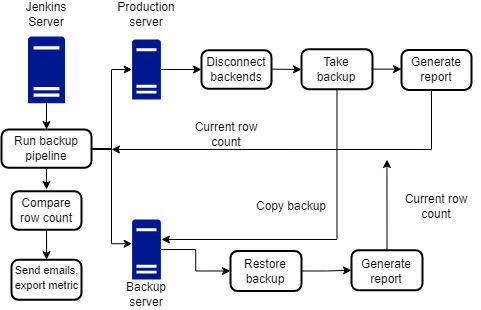
\includegraphics{images/backup.png}
	\caption{Database backup architecture}
	\label{fig:figure4_2}
\end{figure}

\hspace{1cm}\textbf{{\large Backup steps:}}
\begin{itemize}
	\item A Pipeline build is triggered in Jenkins server everyday at midnight. 
	\item  The Database server shouldn't receive any requests. So, webserver(tomcat) is disconnected from load balancer(HAproxy) and waits for one minute to ensure no user request is waiting in server's buffer.
	\item Using mysqldump, specified database is backedup into a file named with mysql-backup-date.sql. 
	\item On production server, pipeline generates a report with details such as total number of rows across all tables in the tables and with per row count with date as each row in a log file, total row count is made available in Jenkins server to later compare with restored row count.
	\item After generating report, the backup file is then copied to backup server using SCP.
	\item On the backup server, the copied backup file is restored and report is generated in backup server and row count is also made available with Jenkins server to be compared with original data.
	\item After restoration, the pipeline code checks for the consistency by comparing total row counts from production server and backup server.
	\item Based on the consistency check, a meaningful metric(pre-defined with custom message with flags) is then exposed using pushgateway to prometheus and a post action is performed based on the backup status.
\end{itemize}


\newpage
\chapter{Result}
\section{Result}
\par Although complete Installation,Configuration,Deployment pipeline is used to deploy for newly assigned projects or for configuring additional server . It has not yet been extensively used, but tested. Deployment pipeline is being used daily as well as backup pipeline which executes everyday and the following are the output screenshots of thier execution.

\section{Sample Output Screenshots}
\textbf{{\large Console output for complete pipeline}}
\begin{figure}[H]
    \centering
    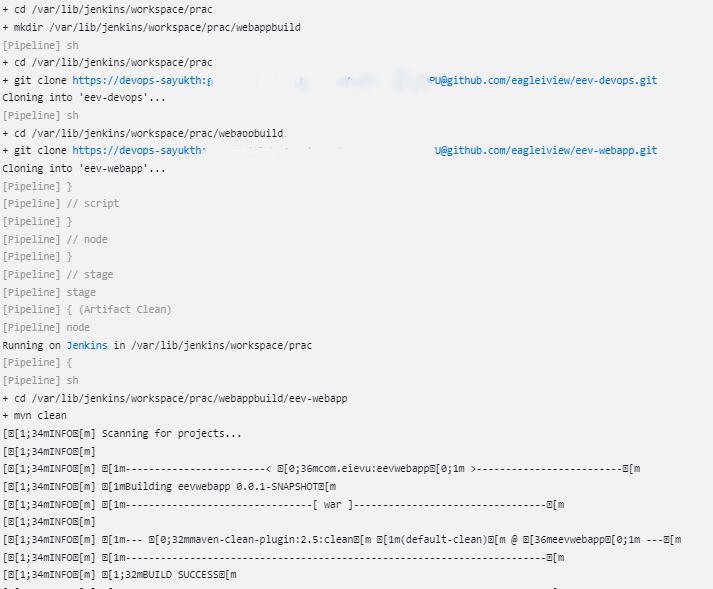
\includegraphics[width=145mm , height = 90mm]{all-deployment-console.png}
    \caption{Stage view for mySQL backup pipelines}
    \label{fig:figure5_1}
\end{figure}
\textbf{{\large Stage view output for deployment pipeline}}
\begin{figure}[H]
    \centering
    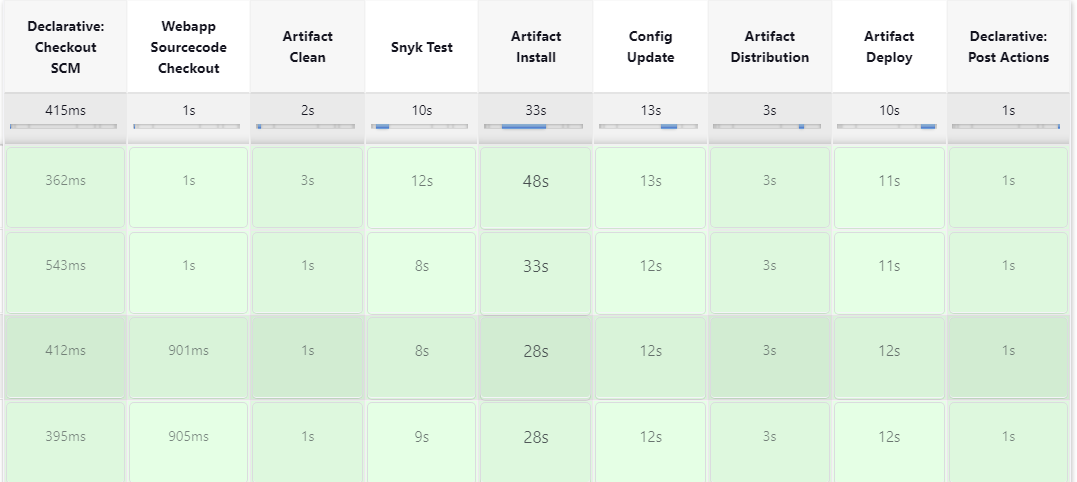
\includegraphics[width=150mm , height = 65mm]{deployment-stages.png}
    \caption{Stage view for only deployment pipelines}
    \label{fig:figure5_1}
\end{figure}
\textbf{{\large Stage view output for Backup pipeline}}
\begin{figure}[H]
    \centering
    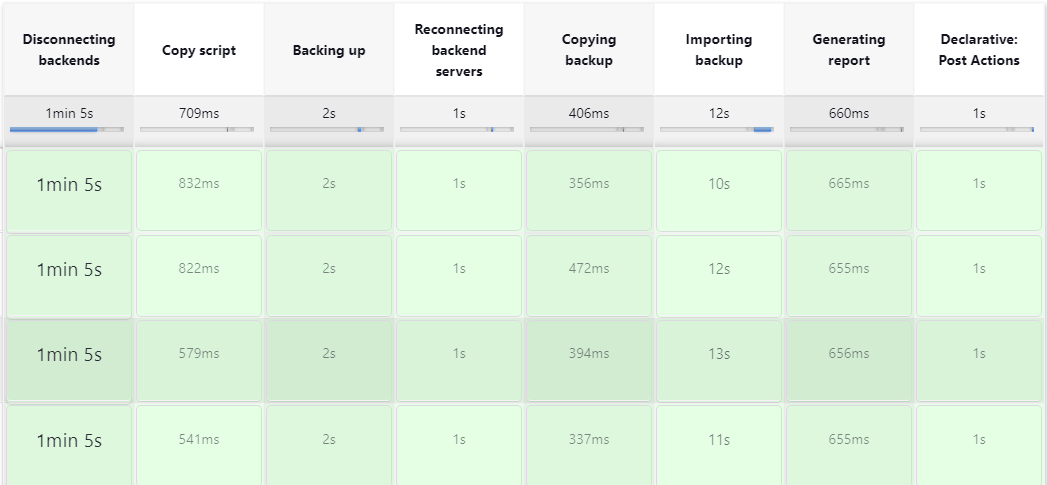
\includegraphics[width=150mm , height = 65mm]{backup-stages.png}
    \caption{Stage view for mySQL backup pipelines}
    \label{fig:figure5_1}
\end{figure}

\section{Requirements}
\subsection{Software Requirements}
\begin{itemize}
\item{Visual studio code editor}
\item{Python3 or above}
\item{Git/Github}
\end{itemize}

\subsection{Hardware Requirements}

\begin{itemize}
\item{Ubuntu 22.04}
\item{4 GB RAM}
\item{20 GB Free Disk Space}
\item{X86 64-bit CPU(Intel/AMD Architecture)}
\end{itemize}


\newpage
\chapter{Future Scope}
\textbf{Enhanced Scalability and Efficiency: }Implementing a robust DevOps automation framework will significantly enhance scalability by enabling automated stack installation, configuration, and version-specific deployments. This will streamline processes, reduce manual efforts, and increase efficiency in managing software development and operations. \\
\textbf{Advanced Security Measures: } The inclusion of security-focused systemd configurations and continuous monitoring using Prometheus and Grafana will bolster system security and visibility. Future enhancements may involve integrating additional security tools and conducting regular security audits to address emerging threats and vulnerabilities. \\
\textbf{Continuous Improvement and Adaptability: }The use of Jenkins for continuous integration and continuous delivery (CI/CD) within the automation framework allows for continuous improvement and adaptability. Future work may involve optimizing Jenkins pipelines, incorporating new plugins, and adopting best practices to ensure efficient and scalable CI/CD workflows. \\
\textbf{Data Integrity and Disaster Recovery: }Automation of data backup processes for MySQL and ScyllaDB databases, along with verification checks and alerting mechanisms, ensures data integrity and enables timely response to potential issues. Future enhancements may include implementing advanced disaster recovery strategies, improving backup efficiency, and integrating with cloud-based backup solutions for enhanced resilience.\\
Overall, the future scope of this DevOps automation framework is promising, with potential advancements in scalability, security, adaptability, and disaster recovery capabilities. By continuously enhancing and refining the framework, organizations can achieve higher levels of efficiency, reliability, and scalability in their software development and operations workflows.



\newpage
\chapter{Conclusion}
\hspace{20pt}  DevOps automation processes, focusing on enhancing efficiency, reliability, and security across software development and operations workflows. Our efforts have centered around implementing a robust DevOps automation framework that includes stack installation, configuration, monitoring, security hardening, and data backup/restoration. This involved developing custom scripts tailored to our specific needs, enabling more rapid deployments and easy upgrades. Additionally, these scripts provide security measures, continuous improvement through Jenkins CI/CD workflows, and the importance of data integrity and disaster recovery, especially in MySQL and ScyllaDB environments. The future scope is promising, with potential advancements in scalability, security, adaptability, and disaster recovery capabilities, paving the way for optimized DevOps practices and enhanced operational excellence.

\newpage
\chapter{References}
\begin{itemize}
\item{https://www.browserstack.com/guide/python-for-devops}
\item{Documentations of respective tools}
\item{https://www.jenkins.io/doc/book/pipeline/}
\item{https://automationqahub.com/how-to-integrate-sonarqube-with-jenkins/}
\item{https://grafana.com/docs/grafana/latest/getting-started/get-started-grafana-prometheus/}
\end{itemize}
\end{document}
